\section{Introduction to Model-Based Testing}

\begin{itemize}
\item Testing could be the most costly phase of a software development project.

\item We can use formal methods to make testing almost automatic, thus changing the cost of testing by the cost of formalization---which is reported to be quite less expensive.

\item Model-based testing (MBT) uses a formal specification to generate test cases and to verify whether they found errors in the program or not.

\item Figure \ref{f:mbt} depicts one of the possible MBT methodologies, a part of which is implemented by Fastest. The methodology is based on \cite{Stocks2}, \cite{Horcher} and \cite{Stocks}.

\item Testing starts by writing a model of the software under test.

\item At the beginning, the model is used to generate test cases.

\item At the end, the model is used as an oracle.

\item The process is very automatic if we have the model.

\item The current version of Fastest only implements the {\it generation} phase of Figure \ref{method}.

\item Fastest is more suitable for unit testing.

\item {\bf The MBT methodology implemented by Fastest, called Test Template Framework (see next section), uses Z formal specifications.}
\end{itemize}

\begin{figure}[h]
\begin{center}
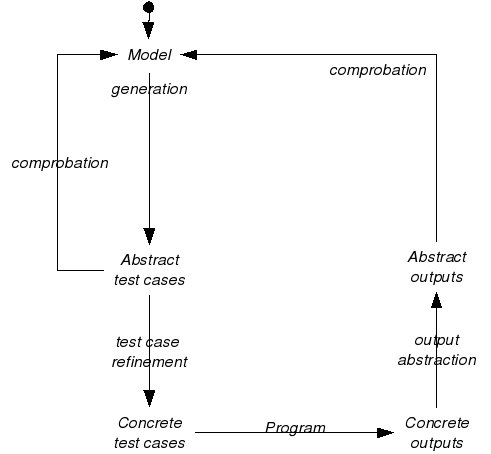
\includegraphics[scale=.9]{testing-func-01.png} 
\caption{\label{f:mbt}Model-based testing methodology: general view.}
\end{center}
\end{figure}







